\section{Recursos Didáticos}

Além dos módulos de cálculo, o DCOU incorpora uma camada de recursos voltados ao aprendizado conceitual, que diferenciam a ferramenta de uma simples calculadora. Esses recursos articulam cada resultado numérico ao seu fundamento teórico e ao fenômeno físico correspondente, apoiando estudantes e engenheiros em formação. As subseções a seguir descrevem o glossário técnico, as explicações teóricas embutidas, as visualizações interativas, os cenários de exemplo e as trilhas de aprendizagem.

\subsection{Glossário}

O glossário reúne 49 termos técnicos organizados em oito categorias (\textit{Hidráulica}, \textit{Dimensionamento}, \textit{Bombas}, \textit{Reatores}, \textit{Componentes}, \textit{Balanço}, \textit{Termodinâmica} e \textit{Transferência de calor}), cada um acompanhado de definição e, quando pertinente, da equação correspondente renderizada matematicamente por meio da biblioteca \textit{KaTeX}. Um campo de busca filtra os termos em tempo real, e as categorias se reorganizam dinamicamente conforme os resultados, permitindo que o estudante localize rapidamente conceitos como número de \textit{Reynolds}, fator de atrito de \textit{Darcy}, \textit{NPSH} ou equação de \textit{Antoine}. Na interface final, o glossário também passou a atuar como recurso de apoio ao fluxo de navegação, aparecendo integrado ao painel de recursos para que o usuário compreenda o papel dessa área sem sair da experiência principal.

\begin{figure}[H]
    \centering
    \caption{Glossário técnico com busca e equações renderizadas}
    \imgouplaceholder{media/cap7_28_glossario_termos_reynolds.png}
    \fonte{Elaboração própria (2026).}
    \label{fig:glossario}
\end{figure}

\subsection{Explicações Teóricas Embutidas}

Cada calculadora dispõe de blocos teóricos retráteis (``Como funciona''), que apresentam a fundamentação do cálculo sem afastar o usuário da interface. Na versão atual, esses blocos não se limitam às calculadoras escalares de diâmetro, número de \textit{Reynolds}, fator de atrito, diâmetro hidráulico, perda de carga, \textit{NPSH} disponível e altura manométrica: eles também acompanham visualizações específicas, como o diagrama de \textit{Moody}, as curvas de bomba, o mapa de eficiência com \textit{BEP}, o diagrama \textit{T-x-y} binário, o \textit{McCabe-Thiele}, o envelope de fase, a curva de pressão de vapor, o diagrama ternário e os painéis de reatores. Em conjunto, esses blocos reúnem equações, regras de leitura, interpretação física das variáveis e referências bibliográficas coerentes com cada fenômeno \cite{white2018,perry2007,fogler2009,smith2018,mccabe2005,poling2001,seader2016,karassik2008,bell2014}.

\begin{figure}[H]
    \centering
    \caption{Exemplo de explicação teórica embutida em uma calculadora}
    \imgouplaceholder{media/explicacao_teorica.png}
    \fonte{Elaboração própria (2026).}
    \label{fig:explicacao_teorica}
\end{figure}

\subsection{Visualizações Interativas}

Para tornar tangíveis os fenômenos físicos, o \textit{frontend} incorpora uma camada ampla de visualizações contextuais construída em componentes reativos de \textit{SVG}. Essa abordagem permite que os gráficos respondam imediatamente às alterações de entrada e se integrem à mesma arquitetura modular dos formulários e resultados. Atualmente, a aplicação reúne mais de vinte visualizações distribuídas entre gráficos numéricos com eixos padronizados, diagramas conceituais, mapas de processo e indicadores de operação. Entre os exemplos, destacam-se o perfil de velocidade do escoamento; a régua de regime de escoamento e o diagrama de \textit{Moody}; as curvas de perda de carga em função da vazão, a margem de \textit{NPSH} e a decomposição da altura manométrica; os diagramas de \textit{Levenspiel}, \textit{T-x-y}, \textit{y-x}, envelope de fase e \textit{McCabe-Thiele}; além de representações de apoio como o gráfico de \textit{Arrhenius}, o perfil espacial de \textit{PFR}, o mapa de eficiência da bomba, os diagramas ternários, a superfície de propriedades e os fluxos de reciclo e purga. Em conjunto, essas visualizações reforçam a leitura dos resultados e aproximam a interpretação numérica do comportamento físico representado.

O valor didático dessa biblioteca de visualizações está em tornar observáveis relações que, em um cálculo puramente tabular, permaneceriam implícitas. No módulo de escoamento, por exemplo, o perfil de velocidade e a régua de regime ajudam a relacionar o número de \textit{Reynolds} com a forma do escoamento e com a mudança de correlações de atrito. No módulo de bombas, as curvas do sistema, a decomposição da altura manométrica, o indicador de \textit{NPSH} e o mapa de eficiência com destaque para o \textit{Best Efficiency Point} (\textit{BEP}) permitem discutir simultaneamente energia mecânica, perdas, faixa operacional e risco de cavitação. Nos módulos de propriedades e reatores, diagramas como \textit{McCabe-Thiele}, envelope de fase, curva de pressão de vapor, \textit{Levenspiel} e \textit{Arrhenius} transformam resultados intermediários do \textit{backend} em objetos gráficos que favorecem a interpretação física das equações, e não apenas a obtenção do valor final.

\begin{figure}[H]
    \centering
    \caption{Card do perfil de velocidade em duto circular}
    \imgouplaceholder{media/cap7_35_dimensionamento_perfil_velocidade_card.png}
    \fonte{Elaboração própria (2026).}
    \label{fig:viz_perfil_velocidade}
\end{figure}

\subsubsection{Diagrama de Moody}

O diagrama de \textit{Moody} foi incorporado para tornar explícita a relação entre número de \textit{Reynolds}, rugosidade relativa e fator de atrito de \textit{Darcy}. Na interface, o usuário não recebe apenas o valor final de $f$: o ponto operacional é sobreposto à família de curvas, permitindo compreender por que materiais distintos e regimes distintos conduzem a perdas de carga diferentes. Como o \textit{backend} já devolve o \textit{Re} calculado, a rugosidade relativa e o fator de atrito coerentes com a correlação adotada, a visualização permanece rastreável ao modelo hidráulico e favorece a leitura do cálculo em chave física, e não apenas algorítmica \cite{white2018,colebrook1939,swamee1976,haaland1983}.

\subsubsection{Curva da Bomba, Margem de \textit{NPSH} e Mapa de Eficiência}

A curva da bomba e do sistema foi adicionada para discutir o ponto operacional como resultado do equilíbrio entre a energia fornecida pelo equipamento e a resistência hidráulica da instalação. Em vez de apresentar apenas uma altura manométrica calculada, a interface mostra como a interseção entre as curvas se desloca quando a vazão ou as perdas variam, o que reforça a interpretação operacional do problema \cite{fox2011}. Complementarmente, o gráfico de margem de \textit{NPSH} foi incluído para representar visualmente a folga entre \textit{NPSHd} e \textit{NPSHr}, permitindo discutir cavitação de modo imediato; já o mapa de eficiência com destaque para o \textit{Best Efficiency Point} (\textit{BEP}) evidencia se a condição corrente está próxima da região de melhor rendimento ou deslocada para uma faixa menos favorável, inclusive com indicação aproximada da região de cavitação. Nesses casos, o \textit{backend} devolve não apenas valores escalares, mas também a malha de eficiência relativa, a curva do sistema, o ponto de operação e os marcadores críticos que estruturam a leitura didática \cite{karassik2008,fox2011}.

\begin{figure}[H]
    \centering
    \caption{Card da curva da bomba e do sistema}
    \imgouplaceholder{media/cap7_40_bombas_curva_bomba_sistema_card.png}
    \fonte{Elaboração própria (2026).}
    \label{fig:viz_curva_bomba_sistema}
\end{figure}

\begin{figure}[H]
    \centering
    \caption{Card da margem de \textit{NPSH}}
    \imgouplaceholder{media/cap7_41_bombas_margem_npsh_card.png}
    \fonte{Elaboração própria (2026).}
    \label{fig:viz_margem_npsh}
\end{figure}

\begin{figure}[H]
    \centering
    \caption{Card do mapa de eficiência da bomba com destaque do \textit{BEP}}
    \imgouplaceholder{media/cap7_33_bombas_mapa_eficiencia_bep_card.png}
    \fonte{Elaboração própria (2026).}
    \label{fig:viz_bep}
\end{figure}

\subsubsection{Diagrama de Levenspiel}

O diagrama de \textit{Levenspiel} foi mantido como peça central do módulo de reatores porque ele transforma a comparação entre \textit{CSTR} e \textit{PFR} em uma relação geométrica facilmente interpretável pelo estudante. Na implementação atual, o gráfico destaca os pontos operacionais de ambos os modelos e compara a demanda volumétrica associada a uma mesma conversão, deixando visível por que o \textit{PFR} tende a requerer menor volume em cinéticas positivas quando comparado ao \textit{CSTR}. Sua presença no TCC é particularmente importante porque ele não atua como ornamento visual: ele traduz em forma gráfica a própria equação de projeto dos reatores ideais, articulando diretamente cálculo e interpretação \cite{levenspiel2000,fogler2009}.

\begin{figure}[H]
    \centering
    \caption{Card do diagrama de \textit{Levenspiel} comparando reatores \textit{CSTR} e \textit{PFR}}
    \imgouplaceholder{media/cap7_39_reatores_levenspiel_card.png}
    \fonte{Elaboração própria (2026).}
    \label{fig:viz_levenspiel}
\end{figure}

\subsubsection{Gráfico de Arrhenius}

O gráfico de \textit{Arrhenius} foi incluído para apoiar a compreensão da dependência da constante cinética com a temperatura. Ao linearizar a relação entre $k$ e $T$ no plano $1000/T$ versus $\ln(k)$, a visualização permite discutir sensibilidade térmica, energia de ativação e velocidade reacional sem exigir que o estudante permaneça apenas na manipulação simbólica da equação. Seu papel pedagógico é evidenciar que pequenas alterações de temperatura podem produzir mudanças expressivas na taxa de reação, o que se conecta diretamente à análise dos módulos de \textit{CSTR} e \textit{PFR} \cite{fogler2009}.

\begin{figure}[H]
    \centering
    \caption{Card do gráfico de \textit{Arrhenius}}
    \imgouplaceholder{media/cap7_38_reatores_arrhenius_card.png}
    \fonte{Elaboração própria (2026).}
    \label{fig:viz_arrhenius}
\end{figure}

\subsubsection{Perfis Espaciais no \textit{PFR}}

Os perfis espaciais no \textit{PFR} foram adicionados para evitar uma leitura excessivamente agregada do reator tubular. Em vez de resumir o comportamento do sistema a um único ponto de saída, a interface exibe séries de concentração e temperatura ao longo do volume relativo do reator, acompanhadas de um esquema que marca estações intermediárias calculadas pelo \textit{backend}. A mesma família de visualizações inclui o gráfico de conversão em função da razão de reciclo, que mostra como a variação de $R$ altera a conversão prevista para o caso atual e permite comparar diretamente cenários de recirculação. Isso ajuda a consolidar a ideia de que o \textit{PFR} deve ser interpretado como um campo espacial de estados e como um sistema sensível à recirculação, no qual cada posição do reator opera sob composição distinta \cite{fogler2009,levenspiel2000}.

\begin{figure}[H]
    \centering
    \caption{Card dos perfis espaciais de concentração e temperatura no \textit{PFR}}
    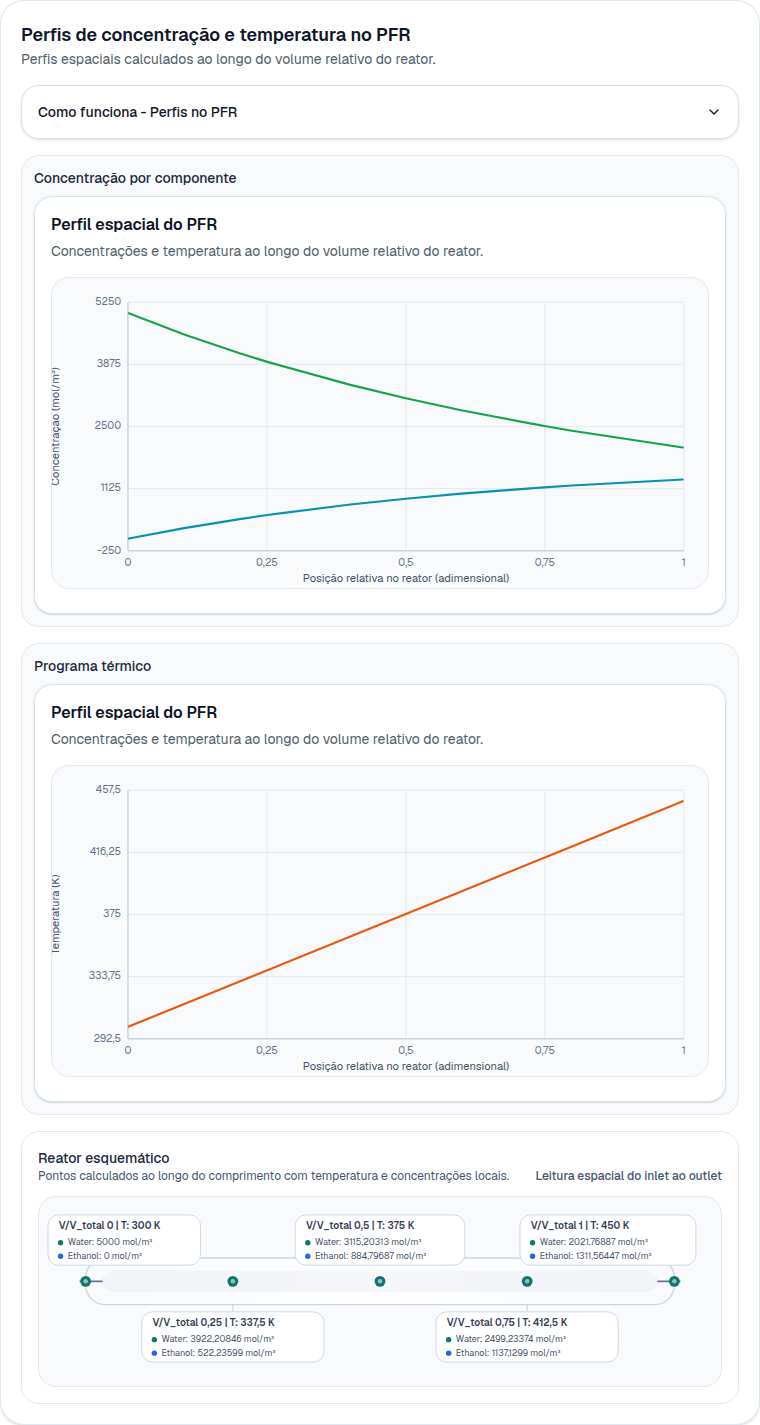
\includegraphics[width=\linewidth,height=0.78\textheight,keepaspectratio]{media/cap7_31_reatores_pfr_perfis_espaciais_card.png}
    \fonte{Elaboração própria (2026).}
    \label{fig:viz_pfr_perfis}
\end{figure}

\begin{figure}[H]
    \centering
    \caption{Card da conversão do \textit{PFR} em função da razão de reciclo}
    \imgouplaceholder{media/cap7_32_reatores_pfr_conversao_reciclo_card.png}
    \fonte{Elaboração própria (2026).}
    \label{fig:viz_pfr_reciclo}
\end{figure}

\subsubsection{Diagrama \textit{T-x-y} Binário}

O diagrama \textit{T-x-y} binário foi incluído para representar o equilíbrio líquido-vapor em misturas binárias a pressão fixa. A presença simultânea das curvas de bolha e de orvalho permite discutir início de vaporização, início de condensação, coexistência entre fases e volatilidade relativa sem depender apenas de tabelas termodinâmicas. Como o \textit{backend} calcula os pontos de equilíbrio e entrega as séries já estruturadas para renderização, o estudante observa o comportamento do sistema a partir de dados consistentes com o mesmo núcleo termodinâmico usado nas demais consultas de propriedades \cite{smith2018}.

\begin{figure}[H]
    \centering
    \caption{Card do diagrama \textit{T-x-y} binário}
    \imgouplaceholder{media/cap7_37_componentes_txy_binario_card.png}
    \fonte{Elaboração própria (2026).}
    \label{fig:viz_txy_binario}
\end{figure}

\subsubsection{Diagrama de McCabe-Thiele}

O diagrama de \textit{McCabe-Thiele} foi incorporado para explicitar a construção gráfica do número teórico de estágios em uma separação binária por destilação. Na aplicação, a curva de equilíbrio, a diagonal, as linhas de enriquecimento e esgotamento, a linha $q$ e os degraus são todos montados a partir dos dados termodinâmicos e operacionais resolvidos no \textit{backend}, o que permite ao usuário relacionar composição de topo, composição de fundo, condição da alimentação e razão de refluxo com a contagem de estágios. O valor didático do gráfico está em mostrar que o resultado de projeto não emerge de uma ``caixa-preta'', mas de uma sequência geométrica interpretável \cite{mccabe2005,smith2018}.

\begin{figure}[H]
    \centering
    \caption{Card do diagrama de \textit{McCabe-Thiele} gerado a partir do equilíbrio binário}
    \imgouplaceholder{media/cap7_30_componentes_mccabe_thiele_card.png}
    \fonte{Elaboração própria (2026).}
    \label{fig:viz_mccabe_thiele}
\end{figure}

\subsubsection{Envelope de Fase e Curva de Pressão de Vapor}

O envelope de fase e a curva de pressão de vapor foram adicionados para apoiar a leitura termodinâmica de limites de estabilidade e mudança de fase. O envelope destaca a fronteira entre regiões de líquido, vapor e coexistência, incluindo marcadores de ponto crítico e ponto tríplice; a curva de pressão de vapor, por sua vez, mostra como a pressão de saturação varia com a temperatura, auxiliando discussões sobre volatilidade, ebulição e risco de cavitação. Em ambos os casos, a utilidade pedagógica está em associar propriedades antes tratadas de forma tabular a regiões operacionais visualmente distinguíveis \cite{poling2001,smith2018}.

\begin{figure}[H]
    \centering
    \caption{Card da curva de pressão de vapor}
    \imgouplaceholder{media/cap7_34_componentes_pressao_vapor_card.png}
    \fonte{Elaboração própria (2026).}
    \label{fig:viz_pressao_vapor}
\end{figure}

\subsubsection{Diagrama Ternário}

O diagrama ternário foi incorporado para representar composições de correntes com três componentes sem a necessidade de introduzir, neste estágio, um módulo completo de separações multicomponentes. Na implementação atual, o \textit{backend} normaliza as frações molares, projeta a corrente no plano ternário e devolve a geometria do triângulo, das linhas-guia e do ponto da corrente pronta para renderização. Didaticamente, isso permite mostrar que cada vértice representa um componente puro, cada lado uma mistura binária e o interior uma composição ternária, o que facilita a leitura de misturas e a preparação conceitual para problemas de extração e equilíbrio mais avançados \cite{seader2016,devoe2014}.

\begin{figure}[H]
    \centering
    \caption{Card do diagrama ternário para uma corrente de três componentes}
    \imgouplaceholder{media/cap7_29_componentes_diagrama_ternario_card.png}
    \fonte{Elaboração própria (2026).}
    \label{fig:viz_ternario}
\end{figure}

\subsubsection{Mapa de Reciclo e Purga}

O mapa de reciclo e purga foi incorporado ao fluxo de balanço de massa para representar graficamente a divisão de uma corrente principal entre retorno ao processo e retirada de produto ou purga. Essa visualização explicita a razão de reciclo adotada no exemplo, evitando que o estudante interprete o reciclo apenas como uma linha tabular e reforçando a relação entre topologia do processo e fechamento de massa.

\begin{figure}[H]
    \centering
    \caption{Card do mapa de reciclo e purga no balanço de massa}
    \imgouplaceholder{media/cap7_36_balanco_fluxos_reciclo_purga_card.png}
    \fonte{Elaboração própria (2026).}
    \label{fig:viz_reciclo_purga}
\end{figure}

\subsubsection{Superfície \textit{T-P} de Propriedades}

Por fim, a superfície \textit{T-P} de propriedades foi adicionada para evidenciar que grandezas termodinâmicas não dependem de forma linear das variáveis de estado. Ao colorir e discretizar o valor de uma propriedade em função de temperatura e pressão, a visualização transforma uma consulta isolada em um campo interpretável, útil para comparar tendências, identificar regiões de maior gradiente e compreender a sensibilidade do modelo termodinâmico às condições impostas. Como essa superfície é construída a partir do mesmo núcleo de propriedades do \textit{CoolProp}, ela reforça a coerência entre cálculo puntual e exploração gráfica \cite{bell2014,poling2001}.

\begin{figure}[H]
    \centering
    \caption{Card da superfície \textit{T-P} de propriedades}
    \imgouplaceholder{media/cap7_42_componentes_superficie_tp_card.png}
    \fonte{Elaboração própria (2026).}
    \label{fig:viz_superficie_tp}
\end{figure}

\subsection{Cenários de Exemplo}

Além das visualizações, o sistema oferece cenários de exemplo providos pela própria \textit{API} para acelerar a exploração didática dos módulos. Em vez de armazenar resultados prontos no \textit{frontend}, esses \textit{endpoints} retornam conjuntos coerentes de entradas para escoamento, dimensionamento, bombas, propriedades de componentes e outros contextos, respeitando os catálogos e limites disponíveis no \textit{backend}. A interface utiliza esses dados para pré-preencher os formulários e, em seguida, executa o mesmo fluxo de cálculo usado em situações reais.

Essa estratégia possui valor pedagógico relevante por dois motivos. Primeiro, reduz a barreira inicial para o estudante, que passa a observar um caso funcional antes de montar um cenário próprio do zero. Segundo, preserva a rastreabilidade entre entradas, equações e visualizações, pois os exemplos não contornam as rotinas de cálculo: eles apenas selecionam condições iniciais representativas, como um caso de transição em número de \textit{Reynolds}, um sistema com margem de \textit{NPSH} explícita ou uma separação binária que justifique a construção de um diagrama de \textit{McCabe-Thiele}.

\subsection{Trilhas de Aprendizagem}

A página inicial organiza o uso dos módulos em três trilhas de aprendizagem, que sugerem uma sequência didática de estudo: \textbf{Transporte de Fluidos} (Tubulações $\rightarrow$ Dimensionamento $\rightarrow$ Escoamento $\rightarrow$ Bombas); \textbf{Reatores Ideais} (Componentes $\rightarrow$ Reatores \textit{CSTR}/\textit{PFR}); e \textbf{Balanço de Massa} (Componentes $\rightarrow$ Balanço). As trilhas orientam o estudante a percorrer os módulos em uma ordem coerente com a construção dos conceitos, em vez de utilizá-los de forma isolada. No desenho atual da interface, essas trilhas convivem com cartões de acesso rápido para os módulos principais, reforçando a intenção de uso de cada área antes da abertura do cálculo.

\begin{figure}[H]
    \centering
    \caption{Trilhas de aprendizagem apresentadas na página inicial}
    \imgouplaceholder{media/cap7_01_tela_inicial_trilhas.png}
    \fonte{Elaboração própria (2026).}
    \label{fig:trilhas}
\end{figure}
